%! Author = lili
%! Date = 6/3/26

\section{Human Practices Documentation Framework}\label{sec:human-practices-documentation-framework}

\subsection{Timeline - Bielefeld-CeBiTec 2024 (Best IHP Winner)}
\subsubsection*{The implementation}
\begin{center}
    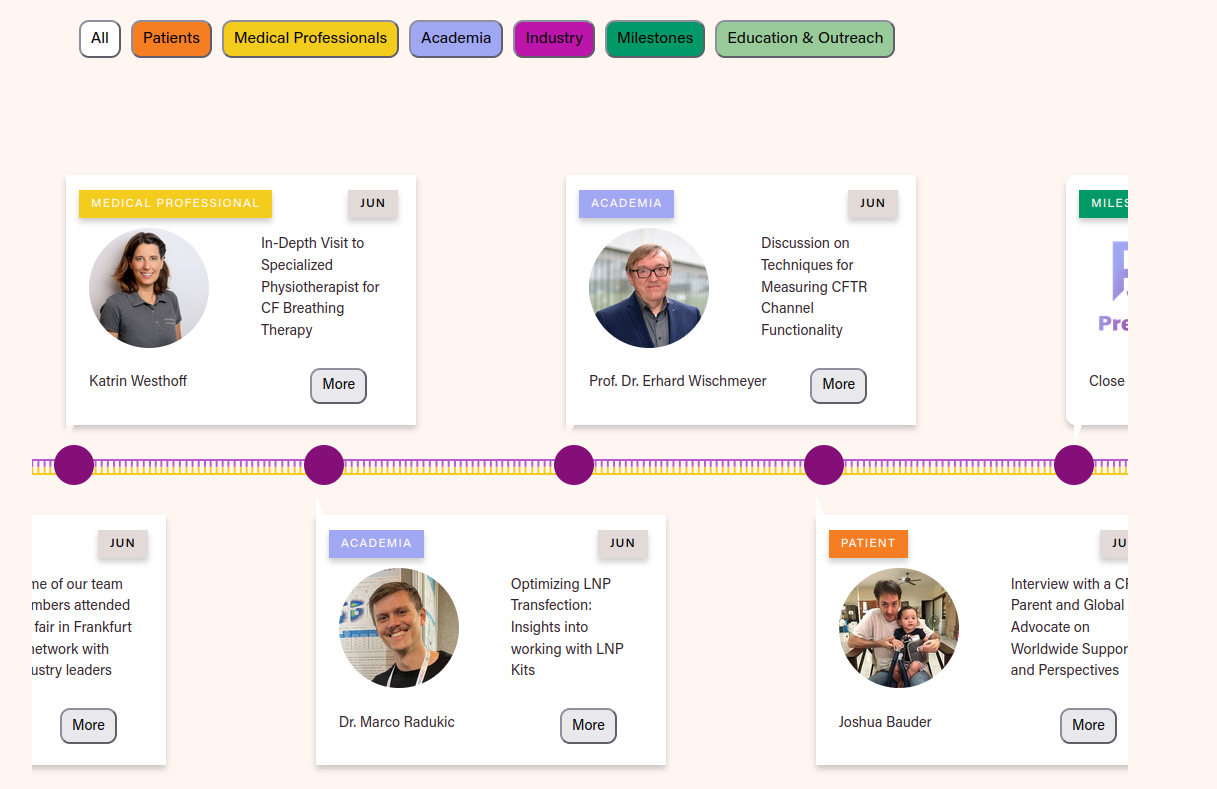
\includegraphics[width=0.8\linewidth]{chapters/images/timelineBielefeld}
\end{center}
\begin{center}
    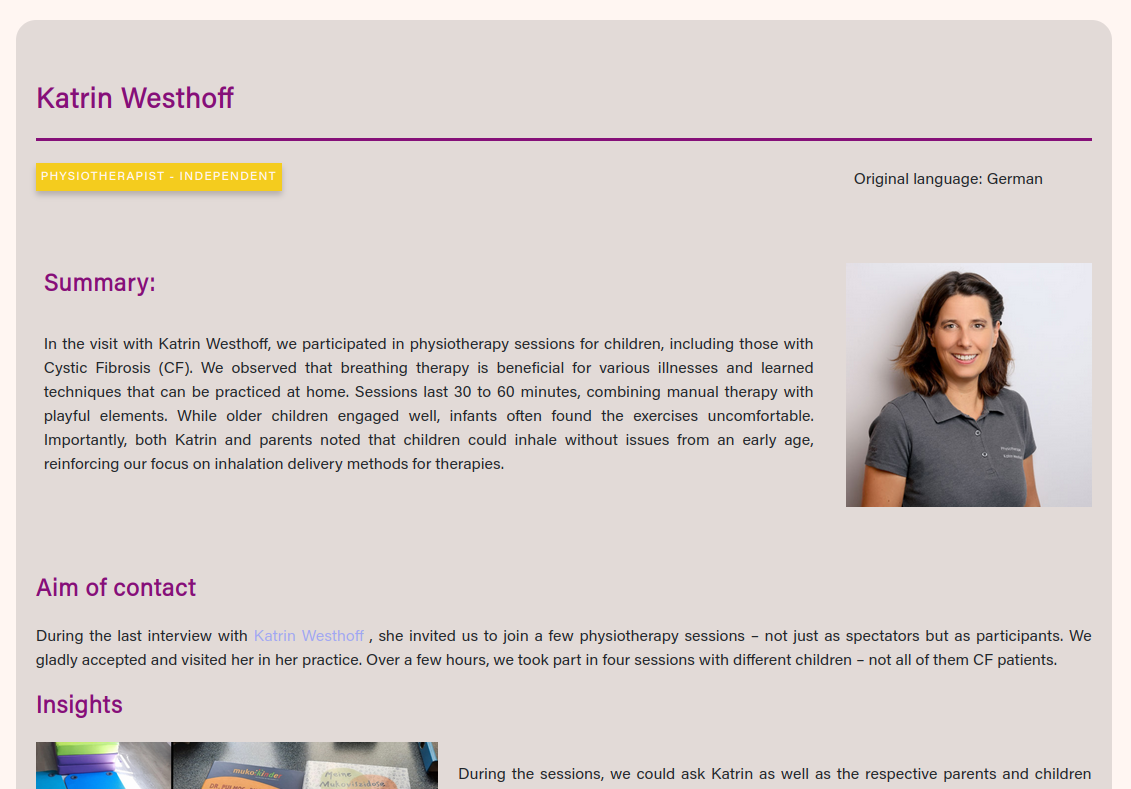
\includegraphics[width=0.7\linewidth]{chapters/images/timelineBielefeldOpen}
\end{center}
\subsubsection*{The structure behind it}
\begin{lstlisting}
export interface TimelineDatenpunkt {
  title?: string; /* Prof. , Dr., ... */
  vorname: string;
  nachnname: string;
  pictureurl: string;
  tag: StakeholderTag;
  heading: string;
  interviewtabid: string;
  summary: string | Array<string> | Array<React.ReactNode>; /* Array<React.ReactNode> for anything that needs HTML, otherwise strings */
  months: string,

  type?: TypeTag; /* only if it is a meta tag */
  affiliation?: string;
  job?: string;
  language?: Language;
  quote?: string;
  quoteVorname?: string; /* If the quote is not from the person the text is about  */
  quoteNachname?: string;
  aimofcontact?: string | Array<string> | Array<React.ReactNode>; /* Array<React.ReactNode> for anything that needs HTML, otherwise strings */
  insights?: string | Array<string> | Array<React.ReactNode>; /* Array<React.ReactNode> for anything that needs HTML, otherwise strings */
  clarification?: string | Array<string> | Array<React.ReactNode>; /* Array<React.ReactNode> for anything that needs HTML, otherwise strings */
  implementation?: string | Array<string> | Array<React.ReactNode>; /* Array<React.ReactNode> for anything that needs HTML, otherwise strings */
  pictureurl_interview?: string;  /* Picture that goes into the paragraph "Insights"  */
  pictureurl_aim?: string;  /* Picture that goes into the paragraph "Aim of contact"  */
  pictureurl_implementation?: string;  /* Picture that goes into the paragraph "Implementation"  */
  more_pictures?: Array<string> ;
  references?: React.ReactNode;  /* Has to be HTML Code - we were not using the citation component yet */
  interview?: React.ReactNode;
  text?: string | Array<string> | Array<React.ReactNode> |React.ReactNode ; /* any extra text */
  experton?: string;
}
\end{lstlisting}

The timeline component rendered visual error messages if aspects were missing.
This approach led to the team only having to fill out the data sheet and getting visual feedback for missing info.
No HTML coding required, but possible.

\subsubsection*{Adaptation by DTU Denmark 2025 (Top 10, Best Wiki Nominee)}
\begin{center}
    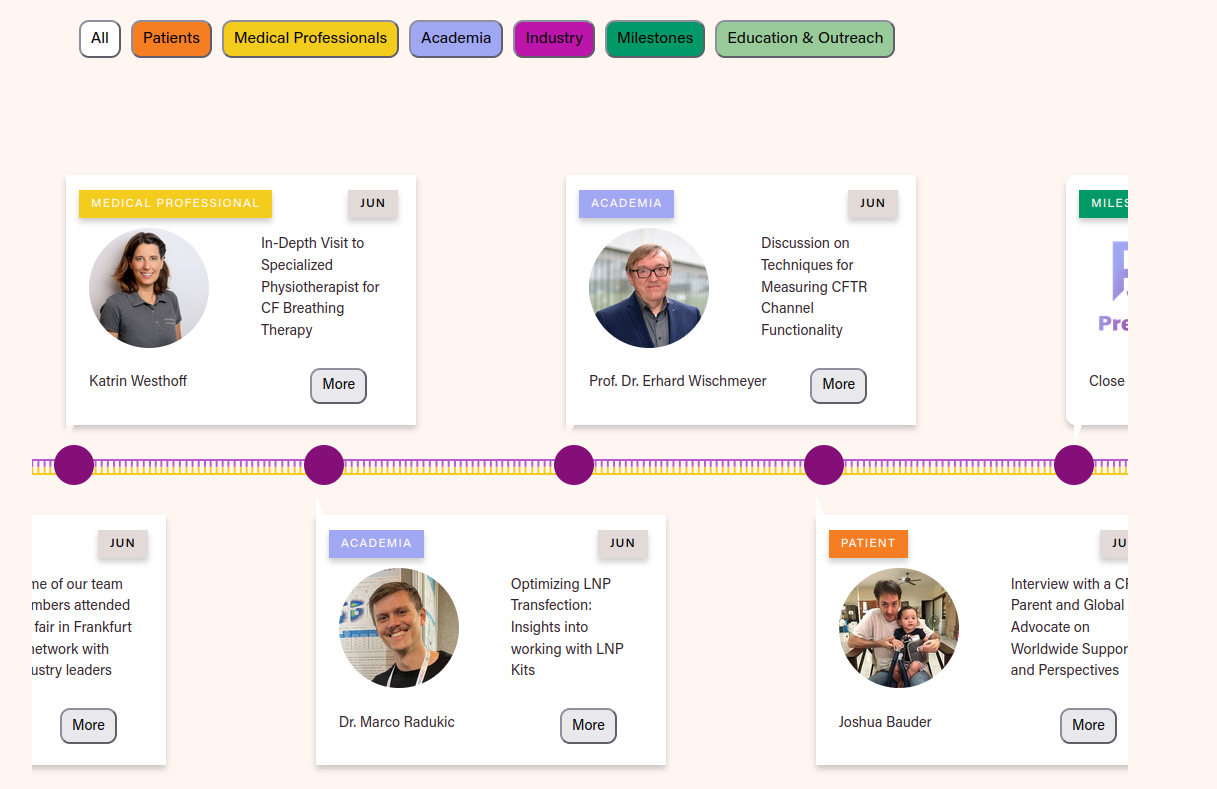
\includegraphics[width=0.8\linewidth]{chapters/images/timelineBielefeld}
\end{center}
\begin{center}
    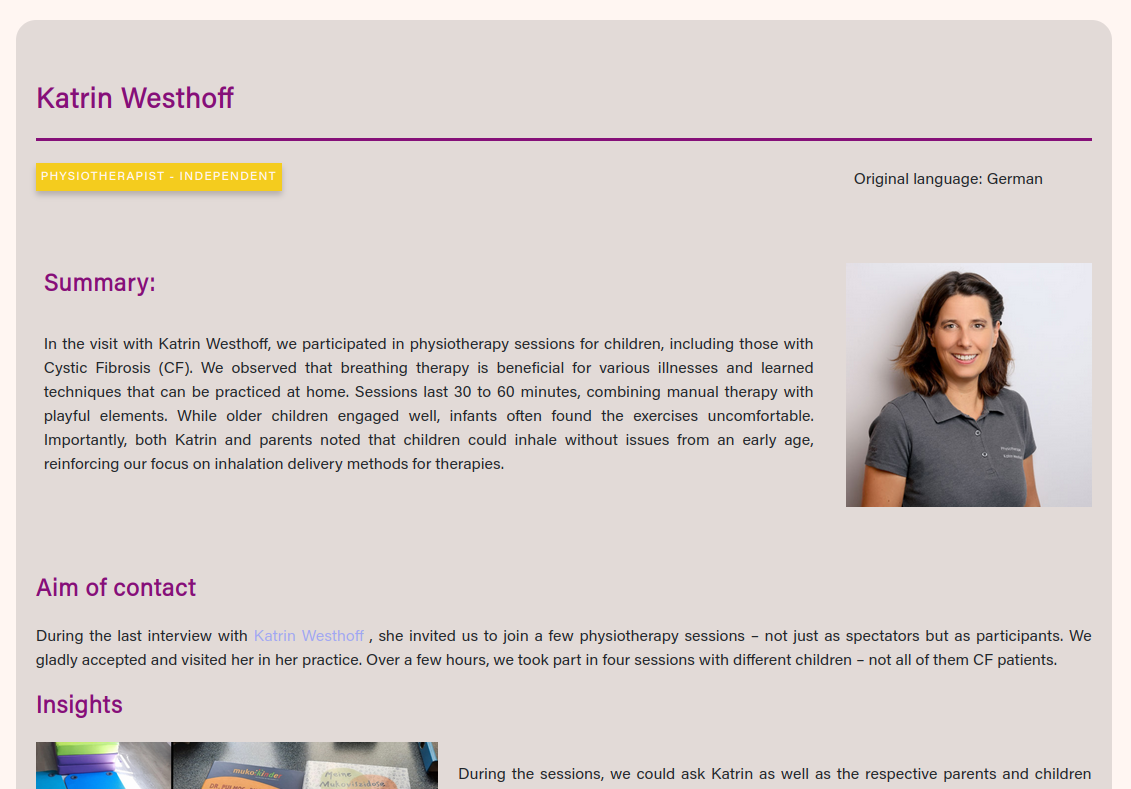
\includegraphics[width=0.7\linewidth]{chapters/images/timelineBielefeldOpen}
\end{center}